%%%%%%%%%%%%%%%%%%%%%%%%%%%%%%%%%%%%%%%%%%%%%%%%%%%%%%%%%%%%%%%%%%%%%%%%%%%%%%%%%%%%%%%%%%%%%%%%
%
% CS484 Written Question Template
%
% Acknowledgements:
% The original code is written by Prof. James Tompkin (james_tompkin@brown.edu).
% The second version is revised by Prof. Min H. Kim (minhkim@kaist.ac.kr).
%
% This is a LaTeX document. LaTeX is a markup language for producing
% documents. Your task is to fill out this document, then to compile
% it into a PDF document.
%
%
% TO COMPILE:
% > pdflatex thisfile.tex
%
% If you do not have LaTeX and need a LaTeX distribution:
% - Personal laptops (all common OS): www.latex-project.org/get/
% - We recommend latex compiler miktex (https://miktex.org/) for windows,
%   macTex (http://www.tug.org/mactex/) for macOS users.
%   And TeXstudio(http://www.texstudio.org/) for latex editor.
%   You should install both compiler and editor for editing latex.
%   The another option is Overleaf (https://www.overleaf.com/) which is
%   an online latex editor.
%
% If you need help with LaTeX, please come to office hours.
% Or, there is plenty of help online:
% https://en.wikibooks.org/wiki/LaTeX
%
% Good luck!
% Min and the CS484 staff
%
%%%%%%%%%%%%%%%%%%%%%%%%%%%%%%%%%%%%%%%%%%%%%%%%%%%%%%%%%%%%%%%%%%%%%%%%%%%%%%%%%%%%%%%%%%%%%%%%
%
% How to include two graphics on the same line:
%
% \includegraphics[width=0.49\linewidth]{yourgraphic1.png}
% \includegraphics[width=0.49\linewidth]{yourgraphic2.png}
%
% How to include equations:
%
% \begin{equation}
% y = mx+c
% \end{equation}
%
%%%%%%%%%%%%%%%%%%%%%%%%%%%%%%%%%%%%%%%%%%%%%%%%%%%%%%%%%%%%%%%%%%%%%%%%%%%%%%%%%%%%%%%%%%%%%%%%

\documentclass[11pt]{article}

\usepackage[english]{babel}
\usepackage[utf8]{inputenc}
\usepackage[colorlinks = true,
linkcolor = blue,
urlcolor  = blue]{hyperref}
\usepackage[a4paper,margin=1.5in]{geometry}
\usepackage{stackengine,graphicx}
\usepackage{fancyhdr}
\setlength{\headheight}{15pt}
\usepackage{microtype}
\usepackage{times}
\usepackage{amsmath, xparse}

% From https://ctan.org/pkg/matlab-prettifier
\usepackage[numbered,framed]{matlab-prettifier}

\frenchspacing
\setlength{\parindent}{0cm} % Default is 15pt.
\setlength{\parskip}{0.3cm plus1mm minus1mm}

\pagestyle{fancy}
\fancyhf{}
\lhead{Homework 2 Questions}
\rhead{CS484}
\rfoot{\thepage}

\date{}

\title{\vspace{-1cm}Homework 2 Questions}


\begin{document}
	\maketitle
	\vspace{-3cm}
	\thispagestyle{fancy}

	\section*{Instructions}
	\begin{itemize}
		\item 4 questions.
		\item Write code where appropriate.
		\item Feel free to include images or equations.
		\item \textbf{Please use only the space provided and keep the page breaks.} Please do not make new pages, nor remove pages. The document is a template to help grading.
		\item If you really need extra space, please use new pages at the end of the document and refer us to it in your answers.
	\end{itemize}

	\section*{Questions}

	\paragraph{Q1:} Explicitly describe image convolution: the input, the transformation, and the output. Why is it useful for computer vision?

	%%%%%%%%%%%%%%%%%%%%%%%%%%%%%%%%%%%
	\paragraph{A1:}
    Image convolution is the act of producing a new pixel value from the values of the corresponding pixel and its neighbors. In other words, the output pixel is defined by the input pixel and the kernel, which defines the transformation from the input pixel (and its neighbors) to the output.

    In computer vision, image convolution is useful for image filtering. By modifying the kernel we use, we can define the correlation between the output pixel and the pixel values and its neighbors. Depending on the kernel, we can make various kinds of changes to an image. We can enhance images by denoising them, or extract information from them by detecting edges, and more.


	%%%%%%%%%%%%%%%%%%%%%%%%%%%%%%%%%%%

	% Please leave the pagebreak
	\pagebreak
	\paragraph{Q2:} What is the difference between convolution and correlation? Construct a scenario which produces a different output between both operations.

	\emph{Please use \href{https://www.mathworks.com/help/images/ref/imfilter.html}{$imfilter$} to experiment! Look at the `options' parameter in MATLAB Help to learn how to switch the underlying operation from correlation to convolution.}

	%%%%%%%%%%%%%%%%%%%%%%%%%%%%%%%%%%%
	\paragraph{A2:}
    The algorithms used between convolution and correlation and very similar yet still different. The equations for correlation and convolution are as follows:
    \begin{align*}
        Correlation: h[m,n] = \sum_{k,l} f[k,l] I[m+k,n+l] \\
        Convolution: h[m,n] = \sum_{k,l} f[k,l] I[m-k,n-l] \\
        \text{Where h is the output matrix, f is the input matrix, and I is the filter}
    \end{align*}

    The equations imply that if the kernel is rotated 180 degrees before applying convolution, it would have the same effect of applying correlation with the original kernel. Therefore it can be inferred that correlation and convolution would yield different results if the kernel is not symmetric along the origin.
    For example, applying the two operations with the following matlab code would produce different outputs.

    \begin{lstlisting}[style=Matlab-editor]
    image = imread('../data/dog.bmp');
    left_shift = zeros(25, 25);
    left_shift(13, end) = 1;
    corr = imfilter(image, left_shift, 'corr');
    figure(1); imshow(corr);
    conv = imfilter(image, left_shift, 'conv');
    figure(2); imshow(conv);
    \end{lstlisting}
    Correlation would shift the image to the left, while convolution would shift the image to the right, as shown from the images below.
    \begin{figure}[h]
        \centering
        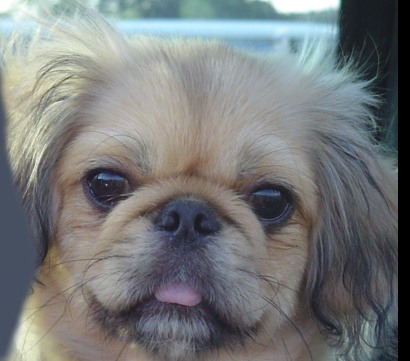
\includegraphics[width=5cm]{corr.jpg}
        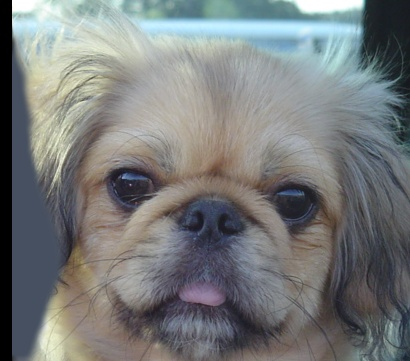
\includegraphics[width=5cm]{conv.jpg}
        \caption{\emph{Left:} Result of Correlation. \emph{Right:} Result of Convolution}
    \end{figure}

	%%%%%%%%%%%%%%%%%%%%%%%%%%%%%%%%%%%

	% Please leave the pagebreak
	\pagebreak
	\paragraph{Q3:} What is the difference between a high pass filter and a low pass filter in how they are constructed, and what they do to the image? Please provide example kernels and output images.

	%%%%%%%%%%%%%%%%%%%%%%%%%%%%%%%%%%%
	\paragraph{A3:}
    A high pass filter and a low pass filter can be expressed in which kernel it uses during convolution. Low pass filters have a smoothing effect, and to implement this kind of behavior one can use a kernel like this:
    \begin{equation}
        \begin{bmatrix}
            1/9 & 1/9 & 1/9 \\
            1/9 & 1/9 & 1/9 \\
            1/9 & 1/9 & 1/9
        \end{bmatrix}
    \end{equation}
    This kernel takes the average of itself and its 8 neighbor pixels to be its own. This reduces the disparity between its pixel value and its neighbors'.
    \begin{figure}[h]
        \centering
        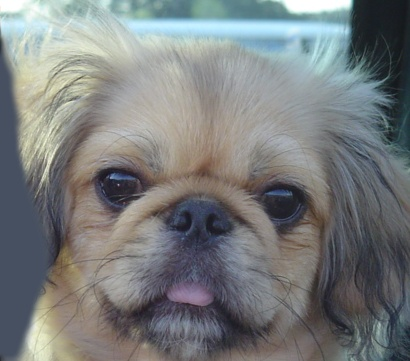
\includegraphics[width=3cm]{original.jpg}
        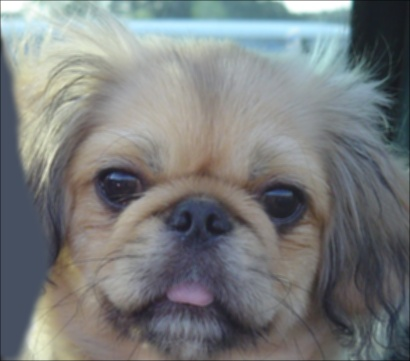
\includegraphics[width=3cm]{lowpass.jpg}
        \caption{\emph{Left:} Original Image. \emph{Right:} Low pass filtered image.}
    \end{figure}


    High pass filters have a sharpening effect, and to implement this kind of behavior one can use a kernel like this:
    \begin{equation}
        \begin{bmatrix}
            -1/9 & -1/9 & -1/9 \\
            -1/9 & 16/9 & -1/9 \\
            -1/9 & -1/9 & -1/9
        \end{bmatrix}
    \end{equation}

    This kernel implements the sharpening effect by amplifying its own pixel value relative to its neighbors. If a certain pixel value has some noise, the noise will be greater in the produced image.
    \begin{figure}[h]
        \centering
        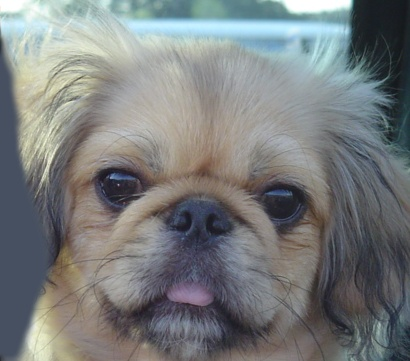
\includegraphics[width=3cm]{original.jpg}
        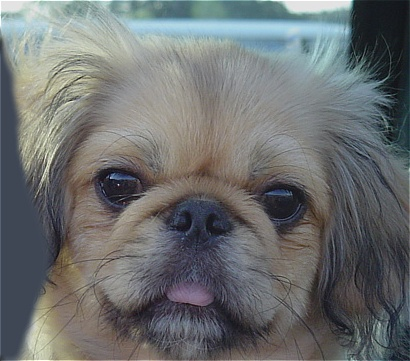
\includegraphics[width=3cm]{highpass.jpg}
        \caption{\emph{Left:} Original Image. \emph{Right:} High pass filtered image.}
    \end{figure}


	%%%%%%%%%%%%%%%%%%%%%%%%%%%%%%%%%%%

	% Please leave the pagebreak
	\pagebreak
	\paragraph{Q4:} How does computation time vary with filter sizes from $3\times3$ to $15\times15$ (for all odd and square sizes), and with image sizes from 0.25~MPix to 8~MPix (choose your own intervals)? Measure both using \href{https://www.mathworks.com/help/images/ref/imfilter.html}{$imfilter$} to produce a matrix of values. Use the \href{https://www.mathworks.com/help/images/ref/imresize.html}{$imresize$} function to vary the size of an image. Use an appropriate charting function to plot your matrix of results, such as \href{https://www.mathworks.com/help/matlab/ref/scatter3.html}{$scatter3$} or \href{https://www.mathworks.com/help/matlab/ref/surf.html}{$surf$}.

	Do the results match your expectation given the number of multiply and add operations in convolution?

	See RISDance.jpg in the attached file.

	%%%%%%%%%%%%%%%%%%%%%%%%%%%%%%%%%%%
    I have calculated the filtering process 100 times for each (filter size, image size) pair and took the average time to plot the 3D graph. There are two variables, the filter size and the image size. Initially, assuming that one variable was fixed, I predicted that the time would increase quadratically. This was because the number of additions and multiplications are roughly calculated as products of widths and heights of the image and filter.

    \begin{align*}
        Multiplications: height_{img} \times width_{img} \times height_{filter} \times width_{filter} \\
        Additions: height_{img} \times width_{img} \times (height_{filter} \times width_{filter} - 1)
    \end{align*}

    Although almost unnoticeable, the trend of lapse time with one variable fixed showed a similar trend with that of a quadratic function, which I initially predicted it to be. When I extended the range of the size of the filter to 3 \textasciitilde31, it became clearer that it was growing more aggressively. Closer to being quadratic than a linear manner.

    \begin{figure}[h]
        \centering
        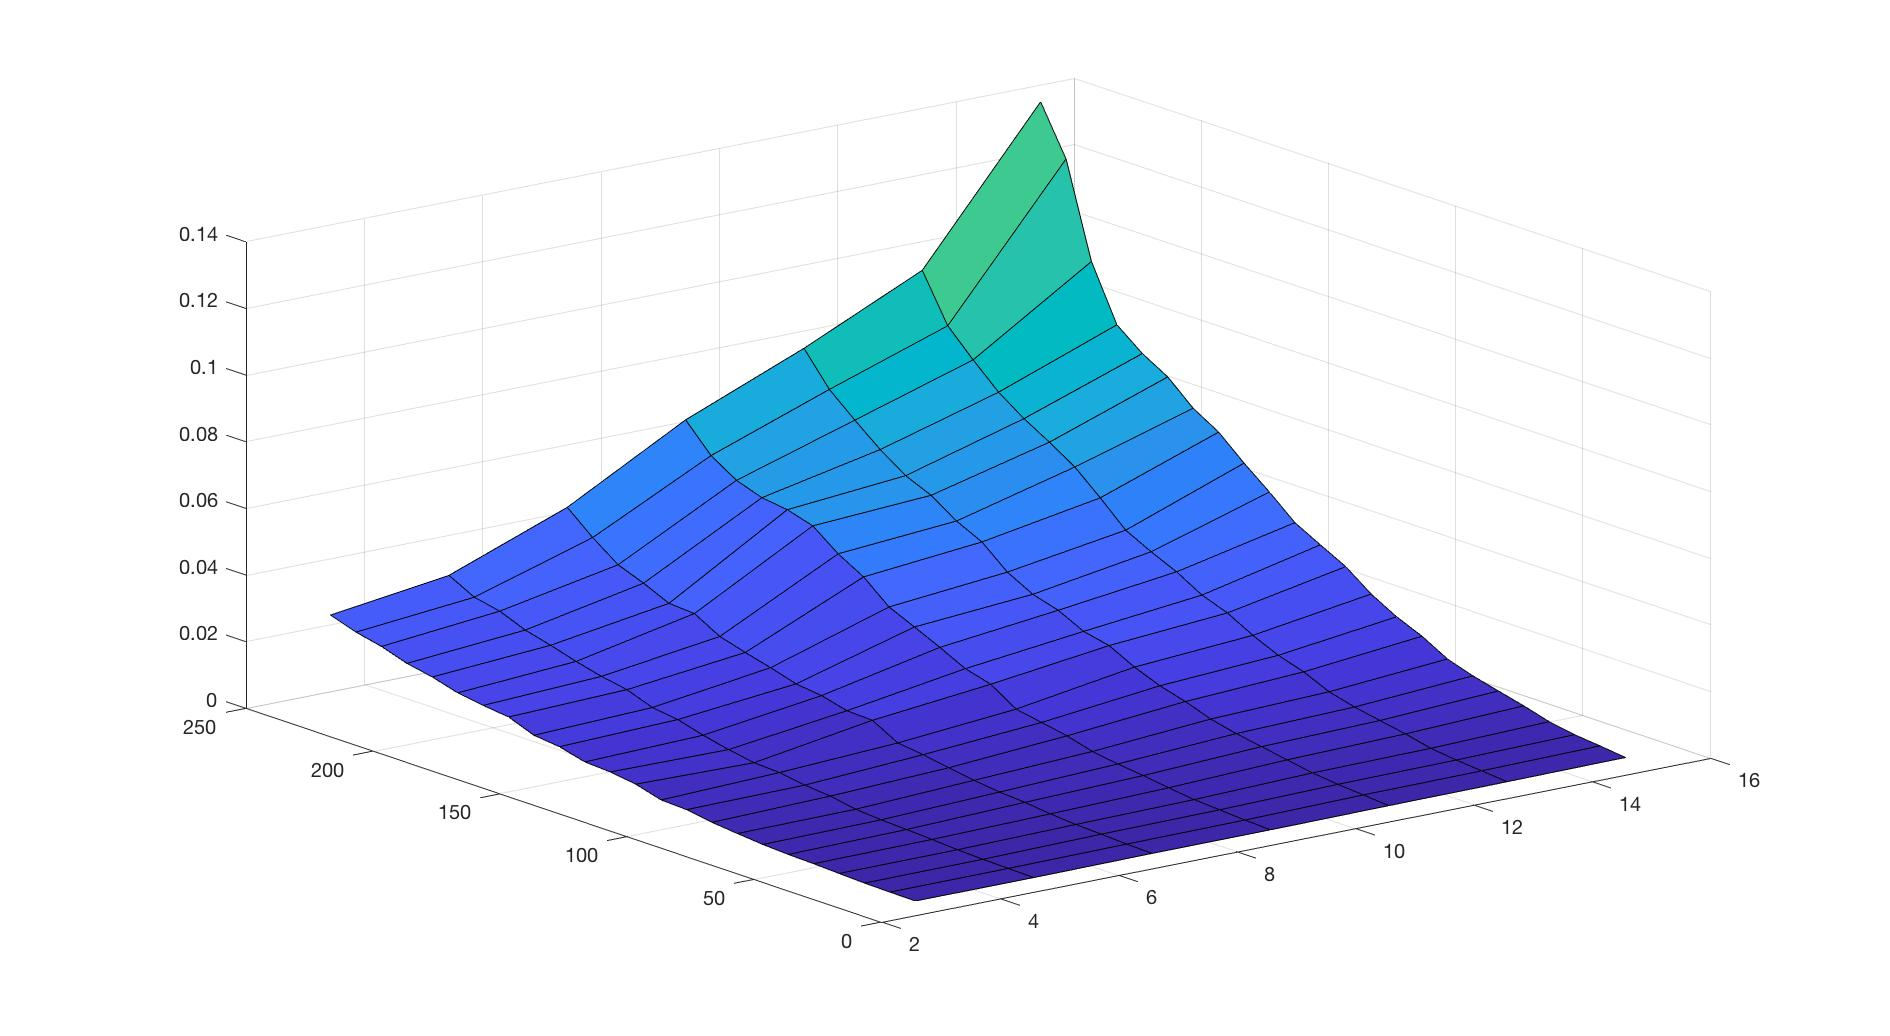
\includegraphics[width=5cm]{q4.jpg}
        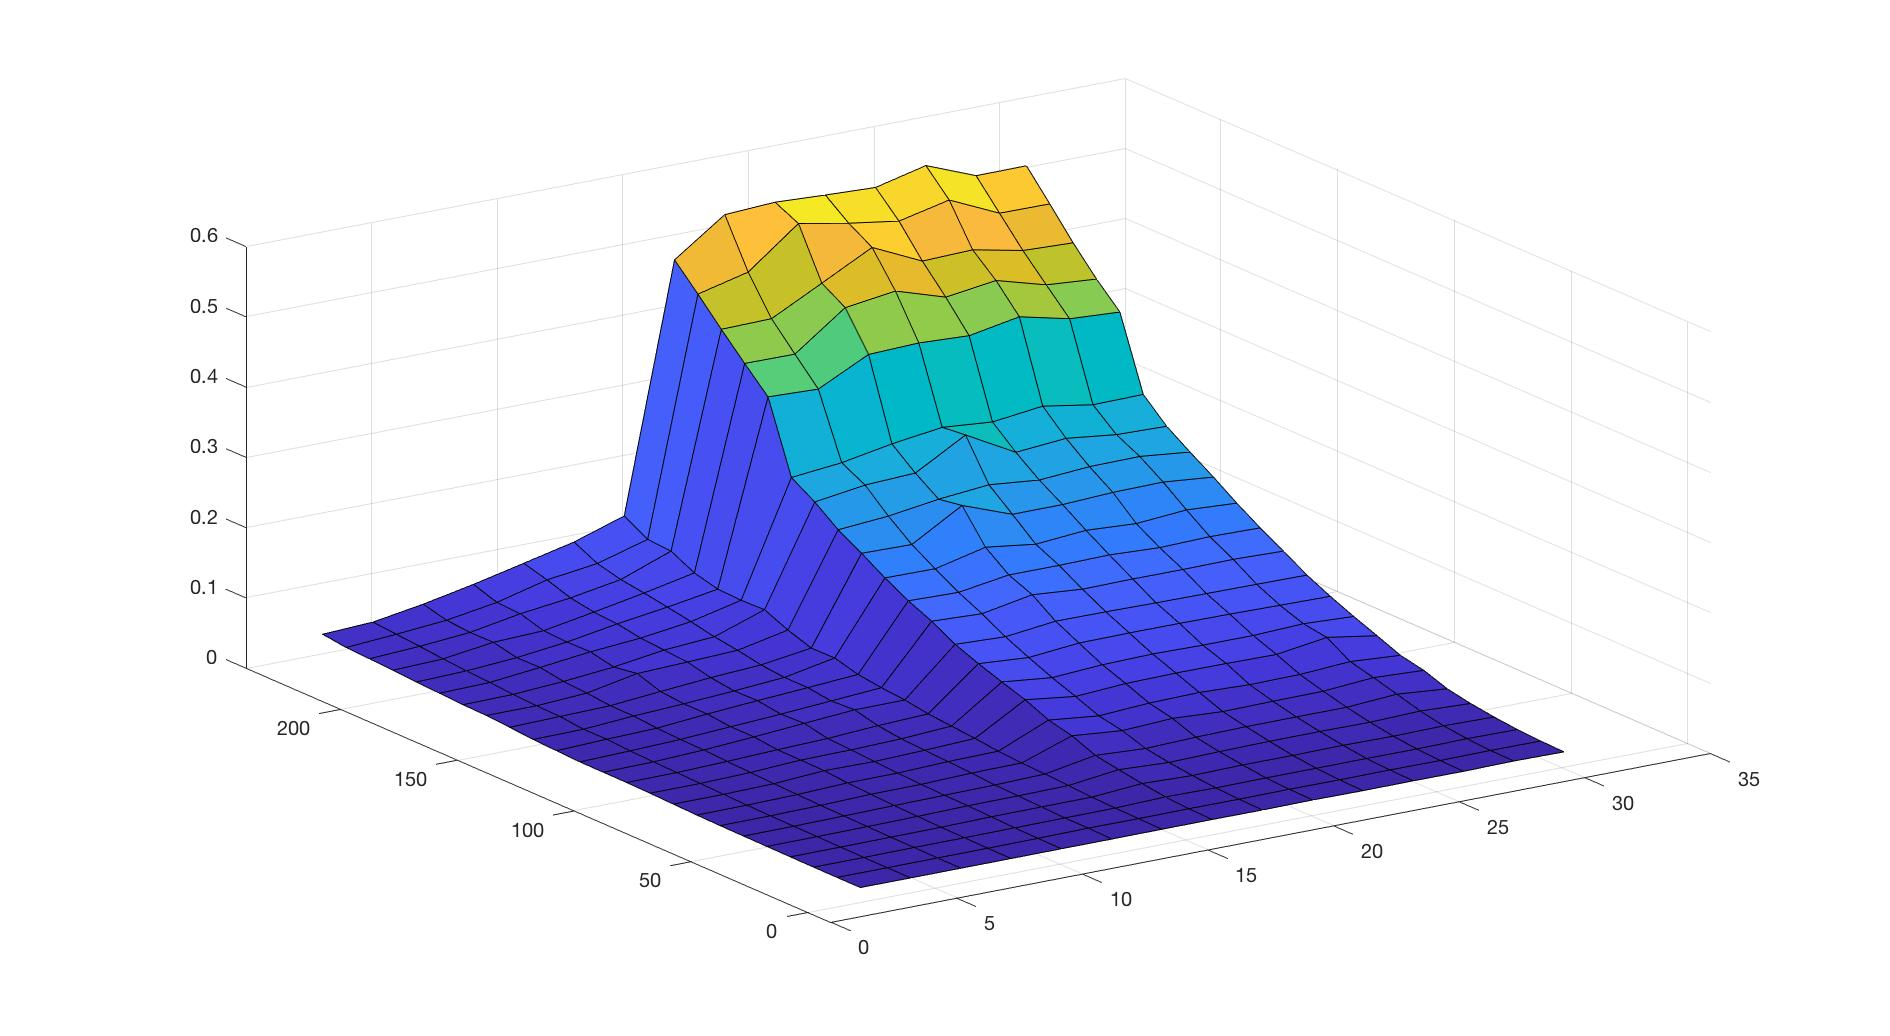
\includegraphics[width=5cm]{q4_extended.jpg}
        \caption{\emph{Left:} Original 3\textasciitilde15 size for filter \emph{Right:} Extended 3 \textasciitilde31 size for filter}
    \end{figure}

	%%%%%%%%%%%%%%%%%%%%%%%%%%%%%%%%%%%


	% If you really need extra space, uncomment here and use extra pages after the last question.
	% Please refer here in your original answer. Thanks!
	%\pagebreak
	%\paragraph{AX.X Continued:} Your answer continued here.
\end{document}
